%
% File acl2017.tex
%
%% Based on the style files for ACL-2015, with some improvements
%%  taken from the NAACL-2016 style
%% Based on the style files for ACL-2014, which were, in turn,
%% based on ACL-2013, ACL-2012, ACL-2011, ACL-2010, ACL-IJCNLP-2009,
%% EACL-2009, IJCNLP-2008...
%% Based on the style files for EACL 2006 by 
%%e.agirre@ehu.es or Sergi.Balari@uab.es
%% and that of ACL 08 by Joakim Nivre and Noah Smith

\documentclass[11pt,a4paper]{article}
\usepackage[hyperref]{acl2017}
\usepackage{times}
\usepackage{latexsym}

\usepackage{url}
\usepackage{graphicx}
\usepackage{booktabs}
\usepackage{color}


\aclfinalcopy % Uncomment this line for the final submission
%\def\aclpaperid{***} %  Enter the acl Paper ID here

%\setlength\titlebox{5cm}
% You can expand the titlebox if you need extra space
% to show all the authors. Please do not make the titlebox
% smaller than 5cm (the original size); we will check this
% in the camera-ready version and ask you to change it back.

\newcommand\BibTeX{B{\sc ib}\TeX}

\newcommand\hm[1]{\textcolor{blue}{#1}}
\newcommand\bs[1]{\textcolor{red}{#1}}

\title{Improving neural tagging with lexical information}

% Author information can be set in various styles:
% For several authors from the same institution:
\author{Beno\^{\i}t Sagot \and H\'ector Mart\'{\i}nez Alonso \\
         Inria\\
       Paris, France\\
\{benoit.sagot,hector.martinez-alonso\}@inria.fr}

\date{}

\begin{document}
\maketitle
\begin{abstract}
  Neural part-of-speech tagging has achieved competitive results with the incorporation of character-based and
  pre-trained word embeddings. In this paper, we show that a state-of-the-art bi-LSTM tagger can benefit from using
  information from morphosyntactic lexicons as additional input. The tagger, trained on several dozen languages, shows a
  consistent, average improvement when using lexical information, even when also using character-based embeddings, thus
  showing the complementarity of the different sources of lexical information. The improvements are particularly
  important for the smaller datasets.
\end{abstract}


\section{Introduction}

Part-of-speech tagging is now a classic task in natural language processing. Its aim is to associate each ``word'' with
a morphosyntactic tag, whose granularity can range from a simple morphosyntactic category, or part-of-speech (hereafter
PoS), to finer categories enriched with morphological features (gender, number, case, tense, mood, person, etc.).

The use of machine learning algorithms trained on manually annotated corpora has long become the standard way to develop
PoS taggers. A large variety of algorithms have been used, such as (in approximative chronological order) bigram and
trigram hidden Markov models \cite{merialdo94,brants96,brants00}, decision trees \cite{schmid94,magerman95}, maximum
entropy Markov models (MEMMs) \cite{ratnaparkhi96} and Conditional Random Fields (CRFs)
\cite{lafferty01,constant12}. Recently, neural approaches have reached very competitive accuracy levels, improving over
the state of the art in a number of settings \cite{plank16}.

As a complement to  annotated training corpora, external lexicons can be a valuable source of information.
First, morphosyntactic lexicons provide a large inventory of (word,~PoS)
pairs. Such lexical information can be used in the form of constraints at tagging time \cite{kim99,hajic00tagging} or
during the training process as additional features combined with standard features extracted from the training corpus
\cite{chrupala08,goldberg09,denis12}.

Second, lexical information encoded in vector representations, known as word embeddings, have emerged more
recently \cite{bengio03,collobert08,chrupala13,ling15,ballesteros15,muller15}. Such representations, often
extracted from large amounts of raw text, have proved very useful for numerous tasks including PoS tagging, in
particular when used in recurrent neural networks (RNNs) and more specifically in mono- or bi-directional, word-level or
character-level long short-term memory networks (LSTMs) \cite{hochreiter97,ling15,ballesteros15,plank16}.

Character-level embeddings are of particular interest for PoS tagging as they generate vector representations that
result from the internal character-level make-up of each word. It can generalise over relevant sub-parts such as
prefixes or suffixes, thus directly addressing the problem of unknown words. However, unknown words do not always follow
such generalisations. In such cases, character-level models cannot bring any advantage. This is a difference with
external lexicons, which provides information about any word it contains, yet without any quantitative distinction
between relevant and less relevant information.

Therefore, a comparative assessment of the advantages of using character-level embeddings and external lexical
information is an interesting idea to follow. However, the inclusion of morphosyntactic information from lexicons into
neural PoS tagging architecture, as a replacement or complement to character-based or pre-computed word embeddings,
remains to be investigated. In this paper, we describe how such an inclusion can be achieved and show, based on
experiments using the Universal Dependencies corpora (version 1.3), that it leads to significant improvements over
\citeauthor{plank16}'s (\citeyear{plank16}) state-of-the-art results.

%\hm{Moreover, lexicon information is qualitatively different from word and character embedding information in that it improves the prediction of A CERTAIN CLASS OF WORDS}

\section{Baseline bi-LSTM tagger}
\label{sec:baselinearchitecture}
As shown by \citet{plank16}, state-of-the-art performance can be achieved using a bi-LSTM architecture fed with word
representations. Optimal performance is achieved representing words using the concatenation of (i) a word vector
$\vec{w}$ built using a word embedding layer, called its {\em word embedding}, and (ii) a representation $\vec{c}$ of
the word's characters, called its {\em character-based embedding} built using a character-level bi-LSTM, which is
trained jointly with the word-level layers. Further improvements can be obtained on most but not all languages by
initialising the word embedding layer with pre-computed word embeddings. We refer to \citet{plank16} for further details.

\section{Integrating lexical information}

We extend this bi-LSTM architecture with an additional input layer that contains token-wise features obtained from a
lexicon. The input vector $\vec{l}$ for a given word is an $n$-hot vector where each active value corresponds to one of
the possible labels in the lexicon. For instance, the English word \textit{house}, which is both a singular noun and a
verb in its base form, will be associated to a 2-hot input vector. Words that are not in the lexicon are represented in
the form of a zero vector. Note there is no need for the morphosyntactic features to be harmonized with the tagset to
predict.

Figure~\ref{fig:schema} shows how the output of this input layer is concatenated to that of the two baseline input
layers, i.e.~the word embedding $\vec{w}$ and (if enabled) the character-based embedding $\vec{c}$. The result of this
concatenation feeds the bi-LSTM layer.

% We do not use the option of multitask learning of the tagger presented by \citeauthor{plank16}'s
% (\citeyear{plank16}), and we use a single bi-LSTM layer instead of multi-layer stacking. While such systems can
% improve the overall results,\footnote{Note however that \citeauthor{plank16}'s (\citeyear{plank16})
%     secondary task---predicting the frequency class of each word---results in better OOV scores but virtually identical
%     overall scores when averaged over all tested languages/corpora.} our goal is to clearly assess the relative
% contribution of information provided by an external morphosyntactic lexicon in contrast to word and character embeddings
% on an already very competitive single-layer baseline.

\begin{figure}
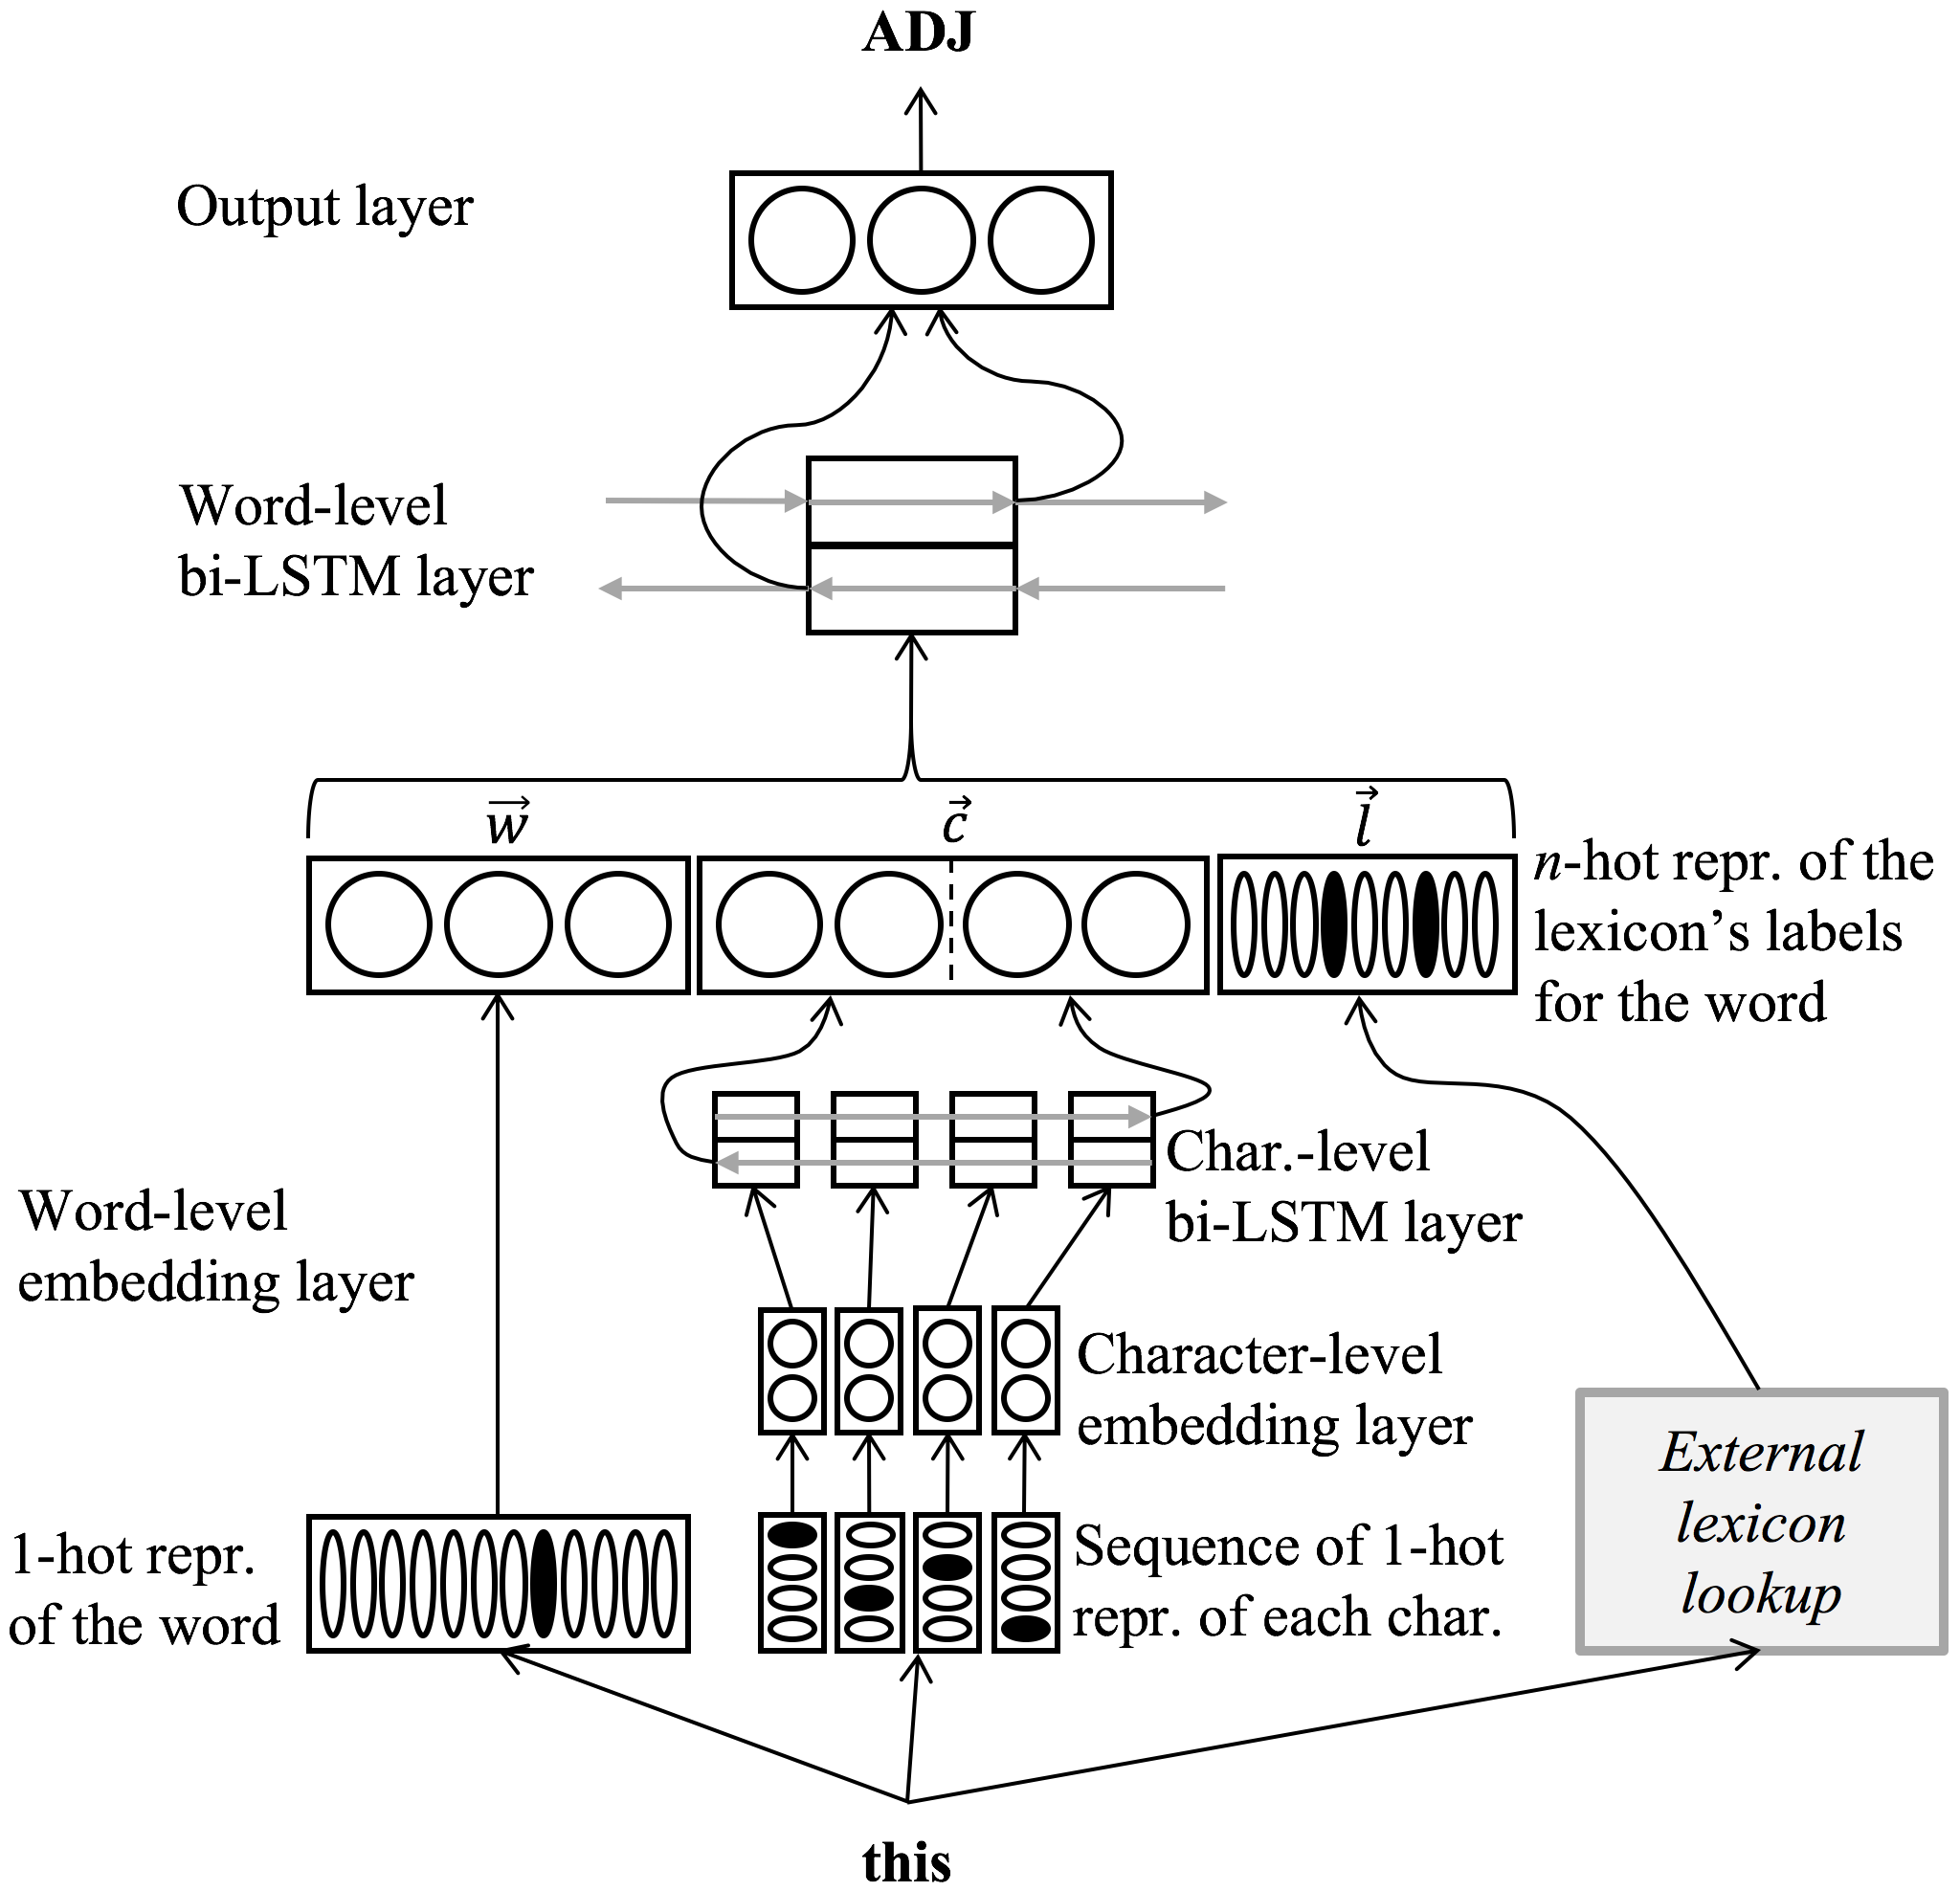
\includegraphics[width=\columnwidth]{emnlp17schemaB2}
%\caption{Schematic representation of the architecture of (a)~\citeauthor{plank16}'s (\citeyear{plank16}) bi-LSTM tagger,
%and (b)~our extension thereof for integrating external morphosyntactic lexical information. Each of these two schemas
%concerns a single word. Connections of the word-level LSTM cells to their counterparts for the preceeding and
%following word are represented with grey arrows.}\label{fig:schema}
\caption{Schema of our extension of \citeauthor{plank16}'s (\citeyear{plank16})
  bi-LSTM tagging architecture for integrating external morphosyntactic lexical information. This schema concerns a
  single word, here ``this.'' Connections of the word-level LSTM cell to its counterparts for the preceeding and
  following word are represented with grey arrows.}\label{fig:schema}
\end{figure}

%\section{Experiments}

\section{Data}

We use the Universal Dependencies (UD) datasets for our experiments. In order to facilitate comparison with
\citeauthor{plank16}'s (\citeyear{plank16}), we performed our experiments on the version 1.3 of UD \cite{ud13}.

\paragraph{Lexicons}

\addtocounter{footnote}{-1}

\begin{table}[t]
\centering
\scriptsize
\begin{tabular}{llrr|rr}
\toprule
 & Name & \#entries & \#tags  & TTR & PG \\
 &  & ($\times 10^3$) &  &  &  \\
\midrule 
ar &   Apertium & 651 & 15 &  yes \\
bg & Multext-East & 53 &12 &  0.18 & yes \\
ca &  Apertium & 379 & 13 &  0.06 & yes \\
cs &  Apertium & 1,875 & 15 &  0.10 & yes \\
da & Apertium & 683 & 15 &  0.19 & yes \\
de & DeLex & 465 & 52 &  0.18 &yes\\
el & Apertium & 47 & 12 &  0.20 & yes \\
en & Apertium & 127 & 12 &  0.09& yes \\
es & Le{\it ff}e &  756 & 34 &  0.12 &yes\\
et & GiellateknoMA & 44 & 12 &  0.23 & yes \\
eu & Apertium\textsubscript{full} & 53 &  14 &  0.22 &  yes \\
fa  & PerLex &  512 & 37 &  0.10 & yes\\
fi & GiellateknoMA & 228 & 13 &  0.29 & yes \\
fr & Le{\it fff} & 539 & 25 & 0.11 &yes\\
ga & inmdb & 114 & 32 &  0.26& yes\\
gl & Apertium & 241 & 12 &  0.12 &no\\
grc  & Diogenes & 1,314 & 18 &  0.20 &no\\
he & Apertium & 268 & 16 &  0.12 & yes\\
hi & Apertium & 159 & 14 &  0.05 & yes\\
hr  & HML   & 1,361 & 22 &  0.21 & yes \\
id & Apertium\textsubscript{full}& 12 & 38 & 0.18 & no   \\
it & Apertium & 278 &14 &  0.10 & yes\\
kk & ApertiumMA& 434 & 16 &  0.48 & no\\
la  & Diogenes & 562 & 16 &  0.31 &no\\
lv & Apertium & 314 & 14  &  0.33& no \\
nl &  Alpino lexicon  & 81 & 65 &  0.14&yes\\
no & Apertium & 2,470 & 13 &  0.11 & yes\\
pl & Apertium & 1,316 &  15 &  0.31 & yes\\
pt & Apertium & 159 & 155 &  0.13 & yes\\
ro &  Multext-East  & 378 & 14 &  0.18 & no \\
ru & Apertium & 4,401 &16&  0.32 & no  \\
sl & Apertium & 654 & 14 &  0.24 &yes\\
sv & Saldo & 1,215 & 214 &  0.17 & yes\\
tr & ApertiumMA & 417 & 14 &  0.32  &no \\
zh & Apertium & 8 & 13 &  0.16 & no \\
\bottomrule
\end{tabular}
\caption{Dataset information. Best per-language lexicon along with its size and number of tags over the UD1.3
  corpora. ``MA'' stands for morphological-analyser-based lexicon. Lexicons based on Apertium and Giellatekno
  data are in their {\em coarse} version unless {\em full} is indicated. Other lexicons
  have been adapted from available resources.\footnotemark{} We also provide the type-token ratio of the 
  corpus (TTR) and whether there were available Polyglot embeddings (PG) to initialize $\vec{w}$.}\label{tbl:lex}
\end{table}

Our sources of lexical information we used are twofold. The first one is the
Apertium\footnote{https://svn.code.sf.net/p/apertium/svn/languages} and the
Giellatekno\footnote{https://victorio.uit.no/langtech/trunk/langs} projects. We used Apertium morphological lexicons
whenever available. For other languages, we downloaded the corresponding monolingual part of OPUS's OpenSubtitles2016
corpus, tokenised it, extracted the 1 million most frequent tokens, and retrieved all their morphological analyses by
the corresponding morphological analyser provided by Apertium (or, failing that, Giellatekno). All these analyses were
then gathered in the form of a lexicon. In a second step, we converted all lexicons obtained using manually crafted
rules, so that each lexical entry contains a (inflected) wordform, a lemma, a Universal
PoS,\footnote{http://universaldependencies.org/u/pos/all.html} and morphological features from the Universal
Features.\footnote{http://universaldependencies.org/u/feat/all.html} We then created two variants of the lexicons
obtained: a {\em coarse} variant in which labels are Universal PoS, and a {\em full} variant in which labels are the
concatenation of the Universal PoS and Universal Features.

We also took advantage of other existing lexicons. For space reasons, we are not able to describe here the
language-specific transformations we applied to some of these lexicons. See Table~\ref{tbl:lex} and its caption for more
information. We determine the best performing lexicon for each language based on tagging accuracy on the development
set. In the remainder of this paper, all information about the lexicons (Table~\ref{tbl:lex}) and accuracy results are
restricted to these best performing lexicons.

Coverage information on the test sets for both the training data and the best external lexicon for each dataset is
provided in Table~\ref{tbl:coverage}.


\paragraph{Pre-computed embeddings}


Whenever available and following \citet{plank16}, we performed experiments using Polyglot pre-computed
embeddings \cite{alrfou13}. Languages for which Polyglot embeddings are available are indicated in Table~\ref{tbl:lex}.

We trained our tagger with and without character-based embeddings, and with or without Polyglot-based
initialisation (when available), both without lexical information and with lexicon information from all available
lexicons, resulting in 4 to 12 training configurations. 


\begin{table}[t]
\centering
\scriptsize
\begin{tabular}{lrrr}
\toprule
Lang & \multicolumn{3}{c}{Coverage (\%)}\\
 & OOTC & OOTC, in Lex. & OOLex\\
\midrule 
ar & 8,0 & 1,0 & 55,0\\
bg & 12,3 & 4,6 & 32,6\\
ca & 4,9 & 2,5 & 20,5\\
cs & 7,0 & 2,9 & 31,7\\
da & 15,6 & 7,3 & 29,0\\
de & 11,9 & 5,3 & 15,1\\
el & 13,4 & 2,0 & 52,7\\
en & 9,1 & 2,6 & 26,1\\
es & 7,3 & 3,5 & 11,3\\
et & 16,9 & 1,4 & 48,9\\
eu & 17,8 & 2,3 & 57,7\\
fa & 8,2 & 2,9 & 31,0\\
fi & 24,4 & 4,0 & 46,0\\
fr & 5,7 & 3,0 & 9,9\\
ga & 22,8 & 7,2 & 66,5\\
gl & 9,9 & 5,9 & 14,9\\
grc & 17,9 & 13,6 & 57,6\\
he & 10,9 & 5,1 & 28,4\\
hi & 4,6 & 1,6 & 17,4\\
hr & 20,9 & 15,1 & 16,5\\
id & 13,8 & 2,4 & 38,3\\
it & 5,7 & 3,4 & 21,4\\
kk & 40,5 & 30,7 & 23,0\\
la & 26,4 & 23,4 & 3,5\\
lv & 36,3 & 16,9 & 42,6\\
nl & 18,8 & 4,4 & 27,6\\
no & 11,2 & 4,0 & 33,0\\
pl & 23,1 & 9,1 & 38,9\\
pt & 8,6 & 3,0 & 29,2\\
ro & 12,1 & 6,8 & 33,1\\
ru & 26,0 & 15,5 & 38,7\\
sl & 19,9 & 11,1 & 28,7\\
sv & 14,9 & 10,4 & 10,4\\
tr & 24,8 & 13,3 & 25,6\\
zh & 12,5 & 0,5 & 66,5\\
\bottomrule
\end{tabular}
\caption{Coverage of the training set and of the best lexicon on the test set for each dataset of the UD~1.3
  corpora. ``OOTC'' stands for ``out of training corpus'' and OOLex for ``out of (external) lexicon''. The ``OOTC, in
  Lex.'' column displays the percentage of words that are not in the training corpus but are covered by the
  lexicon. Best improvements are expected for these words.\label{tbl:coverage}}
\end{table}

\footnotetext{\citealp{bouma00,oliver04,heslin07,borin08,molinero09,sagot10lefff,erjavec10,sagot10perlex,mechura14,sagot14delex}.}

\section{Experimental setup}

\begin{table*}[t]
\centering\scriptsize
\begin{tabular}{l|rrr|rrr|rrr}
\toprule
Language & \multicolumn{3}{c|}{Baseline} & \multicolumn{3}{c|}{With best lexicon} & \multicolumn{3}{c}{Gain when using} \\
 & \multicolumn{3}{c|}{(no lexicon)} & \multicolumn{3}{c|}{(selected on dev, cf.~Tab.~\ref{tbl:lex})} & \multicolumn{3}{c}{best lexicon} \\
 & \multicolumn{1}{c}{$\vec{w}$} & \multicolumn{1}{c}{$\vec{w}+\vec{c}$} & \multicolumn{1}{c|}{$\vec{w}_P+\vec{c}$} & \multicolumn{1}{c}{$\vec{w}+\vec{l}$} & \multicolumn{1}{c}{$\vec{w}+\vec{c}+\vec{l}$} & \multicolumn{1}{c|}{$\vec{w}_P+\vec{c}+\vec{l}$} & \multicolumn{1}{c}{$\vec{w}(+\vec{l})$} & \multicolumn{1}{c}{$\vec{w}+\vec{c}(+\vec{l})$} & \multicolumn{1}{c}{$\vec{w}_P+\vec{c}(+\vec{l})$} \\
\midrule
Arabic (ar) & 93.90 & 95.99 & 96.20 & 94.58 & 96.05 & 96.22 & +0.68 & +0.06 & +0.02\\
Bulgarian (bg) & 94.50 & 98.11 & 97.62 & 96.29 & 98.30 & 97.86 & +1.79 & +0.18 & +0.24\\
Catalan (ca) & 96.14 & 98.03 & 98.17 & 97.58 & 98.21 & 98.26 & +1.44 & +0.18 & +0.09\\
Czech (cs) & 95.93 & 98.03 & 98.10 & 96.74 & 98.46 & 98.41 & +0.81 & +0.43 & +0.31\\
Danish (da) & 90.16 & 95.41 & 95.62 & 94.20 & 96.24 & 96.14 & +4.04 & +0.83 & +0.53\\
German (de) & 87.94 & 92.64 & 92.96 & 91.52 & 93.08 & 93.18 & +3.58 & +0.44 & +0.23\\
Greek (el) & 95.62 & 97.76 & 98.22 & 96.03 & 97.67 & 98.17 & +0.41 & --0.09 & --0.05\\
English (en) & 91.12 & 94.38 & 94.56 & 92.97 & 94.63 & 94.70 & +1.85 & +0.25 & +0.14\\
Spanish (es) & 93.10 & 94.96 & 95.27 & 94.62 & 94.84 & 95.07 & +1.52 & --0.11 & --0.20\\
Estonian (et) & 90.73 & 96.10 & 96.40 & 90.07 & 96.14 & 96.66 & --0.65 & +0.04 & +0.26\\
Basque (eu) & 88.54 & 94.34 & 95.07 & 88.52 & 94.78 & 95.03 & --0.02 & +0.44 & --0.04\\
Persian (fa) & 95.57 & 96.39 & 97.35 & 96.22 & 97.09 & 97.35 & +0.65 & +0.71 & +0.00\\
Finnish (fi) & 87.26 & 94.84 & 95.12 & 88.67 & 94.87 & 95.13 & +1.40 & +0.03 & +0.01\\
French (fr) & 94.30 & 95.97 & 96.32 & 95.92 & 96.71 & 96.28 & +1.62 & +0.74 & --0.04\\
Irish (ga) & 86.94 & 89.87 & 91.91 & 88.88 & 91.18 & 91.76 & +1.94 & +1.31 & --0.16\\
Galician (gl) & 94.78 & 96.94 & --- & 95.72 & 97.18 & --- & +0.94 & +0.24 & ---\\
Ancient Greek (grc) & 88.69 & 94.40 & --- & 89.76 & 93.75 & --- & +1.07 & -0.65 & ---\\
Hebrew (he) & 92.82 & 95.05 & 96.57 & 94.11 & 95.53 & 96.76 & +1.29 & +0.48 & +0.19\\
Hindi (hi) & 95.55 & 96.22 & 95.93 & 96.22 & 96.50 & 96.95 & +0.67 & +0.28 & +1.02\\
Croatian (hr) & 86.62 & 95.01 & 95.93 & 93.53 & 96.29 & 96.34 & +6.91 & +1.28 & +0.41\\
Indonesian (id) & 89.07 & 92.78 & 93.27 & 91.17 & 92.79 & 92.89 & +2.11 & +0.02 & --0.38\\
Italian (it) & 95.29 & 97.48 & 97.77 & 97.54 & 97.81 & 97.88 & +2.26 & +0.33 & +0.11\\
Kazakh (kk) & 72.74 & 76.32 & --- & 82.28 & 82.79 & --- & +9.54 & +6.47 & ---\\
Latin (la) & 85.18 & 92.18 & --- & 90.63 & 93.29 & --- & +5.44 & +1.12 & ---\\
Latvian (lv) & 78.22 & 89.39 & --- & 83.56 & 91.07 & --- & +5.35 & +1.68 & ---\\
Dutch (nl) & 84.91 & 89.97 & 87.80 & 85.20 & 90.69 & 89.85 & +0.29 & +0.72 & +2.05\\
Norwegian (no) & 93.65 & 97.50 & 97.90 & 95.80 & 97.72 & 97.96 & +2.15 & +0.22 & +0.07\\
Polish (pl) & 87.99 & 96.21 & 96.90 & 90.81 & 96.40 & 97.02 & +2.83 & +0.18 & +0.13\\
Portuguese (pt) & 93.61 & 97.00 & 97.27 & 94.76 & 96.79 & 97.11 & +1.15 & --0.21 & --0.16\\
Romanian (ro) & 92.63 & 95.76 & --- & 94.49 & 96.26 & --- & +1.86 & +0.51 & ---\\
Russian (ru) & 84.72 & 95.73 & --- & 93.50 & 96.32 & --- & +8.79 & +0.60 & ---\\
Slovene (sl) & 83.96 & 97.30 & 95.27 & 94.07 & 97.74 & 95.44 & 10.11 & +0.44 & +0.17\\
Swedish (sv) & 92.06 & 96.26 & 96.56 & 95.61 & 97.03 & 97.00 & +3.55 & +0.77 & +0.44\\
Turkish (tr) & 87.02 & 93.98 & --- & 90.03 & 93.90 & --- & +3.01 & --0.08 & ---\\
Chinese (zh) & 89.17 & 92.99 & --- & 89.29 & 93.04 & --- & +0.12 & +0.05 & ---\\
\midrule
Macro-avg. & 90.01 & 94.61 & --- & 92.60 & 95.18 & --- & +2.59 & +0.57 & ---\\
Macro-avg.~w/embed & 91.43 & 95.52 & 95.77 & 93.52 & 95.91 & 95.98 & +2.09 & +0.38 & +0.21\\
\end{tabular}
\caption{Overall results. PoS accuracy scores are given for each language in the baseline
  configuration (the same as \citealp{plank16}) and in the lexicon-enabled configuration. For each configuration, scores
are given when using word embeddings only ($\vec{w}$), word and character-based embeddings ($\vec{w}+\vec{c}$), and word
and character-based embeddings with initialisation of word embeddings with Polyglot vectors ($\vec{w}_P+\vec{c}$). The
 last columns show the difference between lexicon-enabled and baseline configurations.\iffalse As can be seen from the
macro-averaged results, both on all languages and on languages for which Polyglot embeddings were available,
lexicon-enabled configurations perform significantly better than the baseline.\fi{}}\label{tbl:results}
\end{table*}

We use as a baseline the state-of-the-art bi-LSTM PoS tagger \texttt{bilty}, a freely
available\footnote{https://github.com/bplank/bilstm-aux} and ``significantly refactored version of the code originally
used'' by \citet{plank16}. We use its standard configuration, with one bi-LSTM layer, character-based embeddings size of
100, word embedding size of 64 (same as Polyglot embeddings), no multitask learning,\footnote{\citeauthor{plank16}'s
  (\citeyear{plank16}) secondary task---predicting the frequency class of each word---results in better OOV scores but
  virtually identical overall scores when averaged over all tested languages/corpora.} and 20 iterations for training.

We extended \texttt{bilty} for enabling integration of lexical morphosyntactic information, in the way described in the
previous section.%\footnote{We also performed experiments in which the mapping between words and lexical labels was not
%  fixed, but was initialised using the lexical information and then updated during training, as for a standard embedding
%  layer. This resulted in slightly better accuracy scores, but also in a massively increased memory usage, to the extent
%  that it was not intractable in practice for most languages. We therefore decided to stick to a fixed
%  word-to-set-of-lexical-labels mapping.}

For each lexicon-related configuration, we trained three variants of the tagger: (i)~a variant without using
character-based embeddings and standard (zero) initialisation of word embeddings before training, (ii)~a variant with
character-based embeddings and standard initialisation of word embeddings, and (iii)~when Polyglot embeddings are
available for the language at hand, a variant with character-based embeddings and initialisation of the word embeddings
with the Polyglot embeddings. This is deliberately similar to \citeauthor{plank16}'s (\citeyear{plank16}) experimental
setup, in order to facilitate the comparison of results.\footnote{Note that we discarded alternative UD 1.3 corpora
  (e.g.~{\tt nl\_lassysmall} vs.~{\tt nl}), as well as corpora for languages for which we had neither a
  lexicon nor Polyglot embeddings (Old Church Slavonic, Hungarian, Gothic, Tamil).}

\begin{table}[th]
\centering\scriptsize
\begin{tabular}{lrrrr}
\toprule
lang & \multicolumn{2}{c}{$\vec{w_{(P)}}+\vec{c}+\vec{l}$}& \multicolumn{2}{c}{$\Delta$ w.r.t.$\vec{w_{(P)}}+\vec{c}$}\\[1mm]
 & OOTC & OOTC in Lex. & OOTC & OOTC in Lex.\\
\midrule
ar & 82,09 & 94,78 & -0,53 & -0,51\\
bg & 92,79 & 96,84 & 4,67 & 0,98\\
ca & 94,21 & 98,38 & 0,31 & -0,11\\
cs & 90,84 & 96,82 & 5,21 & 0,57\\
da & 88,54 & 95,03 & 3,17 & 0,70\\
de & 86,05 & 87,00 & 3,32 & 0,41\\
el & 89,22 & 96,52 & -1,97 & -0,90\\
en & 78,23 & 89,31 & 3,89 & 1,02\\
es & 76,34 & 79,33 & -1,21 & -1,12\\
et & 88,24 & 94,80 & -1,62 & -0,70\\
eu & 82,02 & 93,26 & -0,09 & -0,41\\
fa & 84,94 & 95,34 & -1,22 & -0,76\\
fi & 85,31 & 92,03 & -0,76 & -0,95\\
fr & 85,50 & 86,35 & 2,25 & 0,43\\
ga & 77,43 & 89,09 & -0,34 & -1,77\\
gl & 85,20 & 91,21 & 21,73 & 5,60\\
grc & 83,71 & 94,40 & 25,16 & 2,00\\
he & 81,36 & 92,25 & -5,81 & -2,61\\
hi & 78,91 & 93,84 & -4,22 & -0,78\\
hr & 90,74 & 88,66 & 1,50 & 0,44\\
id & 86,07 & 90,72 & -1,29 & -0,55\\
it & 89,15 & 96,46 & 1,12 & -0,43\\
kk & 76,89 & 52,59 & 23,53 & -2,96\\
la & 84,51 & 88,89 & 28,95 & 10,53\\
lv & 80,98 & 83,64 & 35,13 & 15,83\\
nl & 69,49 & 78,60 & 12,75 & 8,19\\
no & 92,44 & 96,97 & -0,24 & -0,48\\
pl & 90,48 & 93,95 & -2,65 & -2,04\\
pt & 88,13 & 95,69 & 0,19 & -0,60\\
ro & 88,39 & 95,47 & 23,18 & 3,71\\
ru & 90,49 & 93,80 & 40,87 & 13,05\\
sl & 93,31 & 95,77 & 11,56 & 4,41\\
sv & 92,43 & 93,31 & 3,88 & -0,47\\
tr & 85,33 & 87,33 & 26,68 & 9,13\\
zh & 78,30 & 92,08 & 24,97 & 5,07\\
\midrule
Macro avg. & 85,37 & 90,87 & 8,06 & 1,83\\
\bottomrule
\end{tabular}
\caption{toto}
\end{table}


\section{Results}

Our results show that using lexical information as an additional input layer to a bi-LSTM PoS tagger results in
consistent improvements over 35 corpora. The improvement holds for all configurations on almost all corpora. As
expected, the greatest improvements are obtained without character-based embeddings, with a macro-averaged improvement
of +2.56, versus +0.57 points when also using character-based embeddings. When also using pre-computed embeddings,
improvements are only slightly lower. External lexical information is useful as it covers both words with an irregular
morphology and words not present in the training data.

The improvements are particularly high for the smaller datasets; in the $\vec{w}+\vec{c}$ setup, the three
languages with the highest improvements when using a lexicon are those with smallest datasets.

% Best performing lexicons often have a reduced tagset. It could be that fine-grained distinctions are made using
% character-based embeddings, whereas lexical information is useful for disambiguating between coarse-grained
% PoS. Moreover, larger sets are bound to be sparser and therefore less easily exploitable as additional information.


% While lexicon coverage is important, the best lexicon for a language is not always the one with the highest coverage,
% e.g.~an alternative lexicon for Italian had a coverage of 90\% instead of 78\%. We attribute this variation to
% properties of the tagset but also to properties of which words are indeed covered by the lexicon.


\section{Conclusion}

Our work shows that word embeddings and external lexical information are complementary sources of morphological
information, which both improve the accuracy of a state-of-the-art neural part-of-speech tagger. It also confirms that
both lexical information and character-based embeddings capture morphological information and help part-of-speech
tagging, especially for unknown words.

Interestingly, we also observe improvements when using external lexical information together with character-based
embeddings, and even when initialising with pre-computed word embeddings. This shows that the use of character-based
embeddings is not sufficient for addressing the problem of out-of-vocabulary words.

Further work includes using lexicons to tag finer-grained tag inventories, as well as a more thorough analysis on the
relation between lexicon and training data properties.

Another natural follow-up to the work presented here would be to examine the interplay between lexical features and more
complex neural architectures, for instance by using more than one bi-LSTM layer, or by embedding the $n$-hot lexicon-based
vector before concatenating it to the word- and character-based embeddings.



\bibliography{iwpt17}
\bibliographystyle{acl_natbib}


\end{document}
